\section{Utilities}
\label{sec:utilities}

\begin{description}

\item[btkModifyImageUsingLookUpTable] This program modifies one image using a
look up table defined in a ascii file (2 columns, one for the original values,
one for the final values). Usage: \texttt{-i input\_image\_filename -t
input\_table\_filename -o output\_image\_filename}
  
\item[btkExtractOneImageFromSequence] This program extracts one image from a 4D sequence. Usage: \texttt{-i input\_image\_filename -o output\_image\_filename --image\_index index}

\item[btkNrrdToNifti] This program convert an image from Nrrd file (*.nhdr and *.nrrd) to a Nifti file (*.nii or *.nii.gz). The conversion of a DWI image is possible by using the option \texttt{-d}. Usage: \texttt{-i input.nhdr -o output.nii.gz}. Usage for DWI sequence: \texttt{-i input.nhdr -o output.nii.gz -g gradients.bvec -d}.

\item[btkNiftiToNrrd] This program convert a diffusion sequence in nifti
format\footnote{Currently there is no nifti standard for DWI, so DW images are
saved as a standard nifti sequence (*.nii, *.nii.gz) and two text files
containing the b-values (.bval) and the gradient directions (.bvec).}  to the
nrrd format (*.nhdr). 

Usage: \texttt{-i input -o output.nhdr}

The list of optional parameters can be obtained by \texttt{btkNiftiToNrrd
--help}

\item[btkSetStandardCoorSystem] It transforms an image to a coordinate
system with identity direction and origin at the center of the image
(by default, a linear interpolation is used).

Usage: \texttt{btkSetStandardCoorSystem -i image -o output -d dimension}. The
argument $-d$ specifies the image dimension (3 for images and 4 for sequences). 
\\

  \item[btkReorientImageToStandard] Sometimes it is useful
to reorient the image to the standard orientation. This is necessary with fetal
images since in general the fetus is in a random orientation with respect to the
scanner. To do this with BTK, before it is necessary to convert the image
to a coordinate system by using \texttt{btkSetStandardCoorSystem}.

Usage: \texttt{btkReorientImageToStandard -i image -o output -l landmarks}.
\texttt{landmarks} is a text file containing points that define the left-right
and the posterior-anterior directions. The points $l$ and $r$ define the left
$\rightarrow$ right direction, and the points $p$ and $a$ define the posterior
$\rightarrow$ anterior direction. Such file can be easily generated by using
Slicer\footnote{http://www.slicer.org} as follows:

\begin{enumerate}
\item Open the high-resolution image by using the \textit{Volume} module.
\item Toogle on the visibility of all slices in the 3D view. This allows to
identify the left and right sides of the brain in the 2D views.
\item Place the landmarks $l$, $r$, $p$, and $a$ in this order by using
\texttt{[p]}.
\item Save the file (*.fcsv) by using the menu File $\rightarrow$ Save.
\end{enumerate}


\begin{figure}[t]
\centering
\begin{tabular}{ccc}
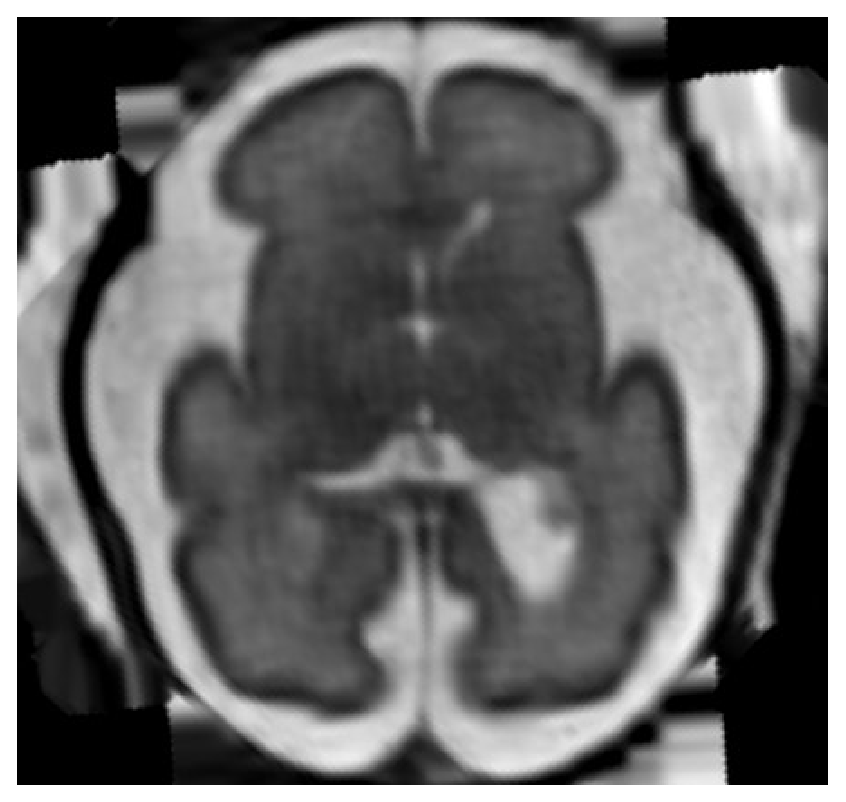
\includegraphics[width=0.3\columnwidth]{hr_axl.eps}&
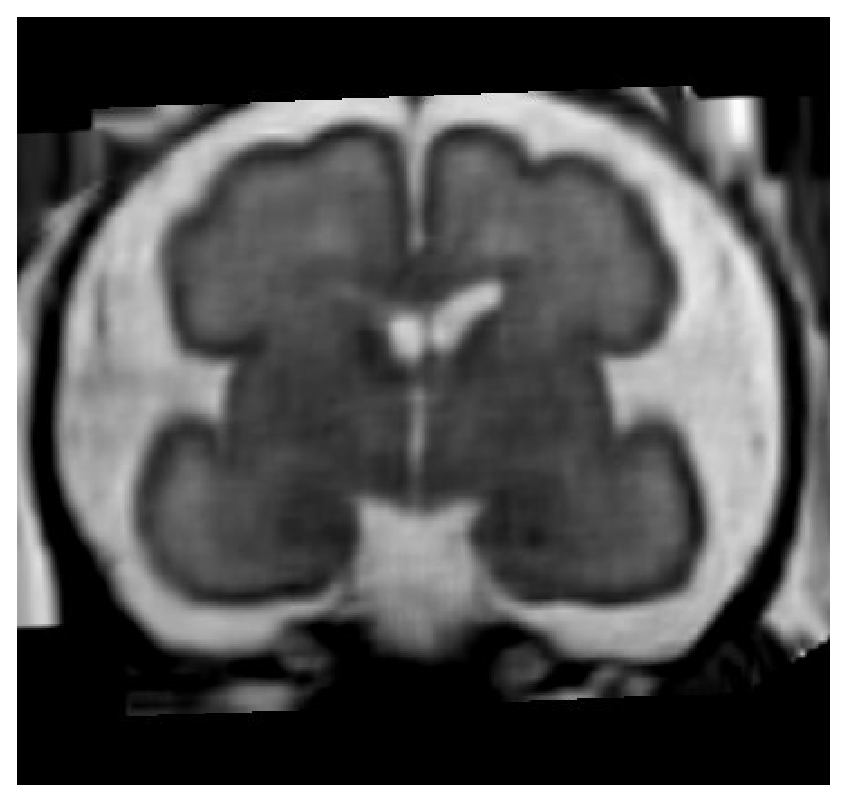
\includegraphics[width=0.3\columnwidth]{hr_cor.eps}&
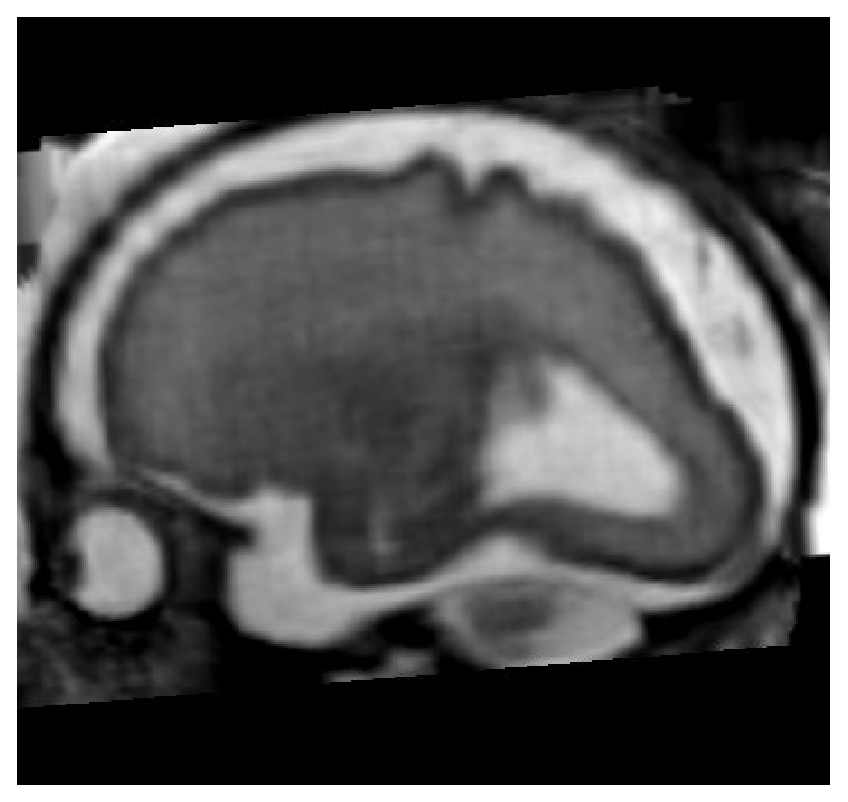
\includegraphics[width=0.3\columnwidth]{hr_sag.eps}\\
{(a)}&{(b)}&{(c)}\\
\end{tabular}
\caption{Example of an anatomical reconstruction of a fetal brain by using
\texttt{btkImageReconstruction}. (a) axial, (b) coronal, and (c) sagital view.}
\label{fig:reconstruction}
\end{figure}

\begin{figure}[t]
\centering
\begin{tabular}{cc}
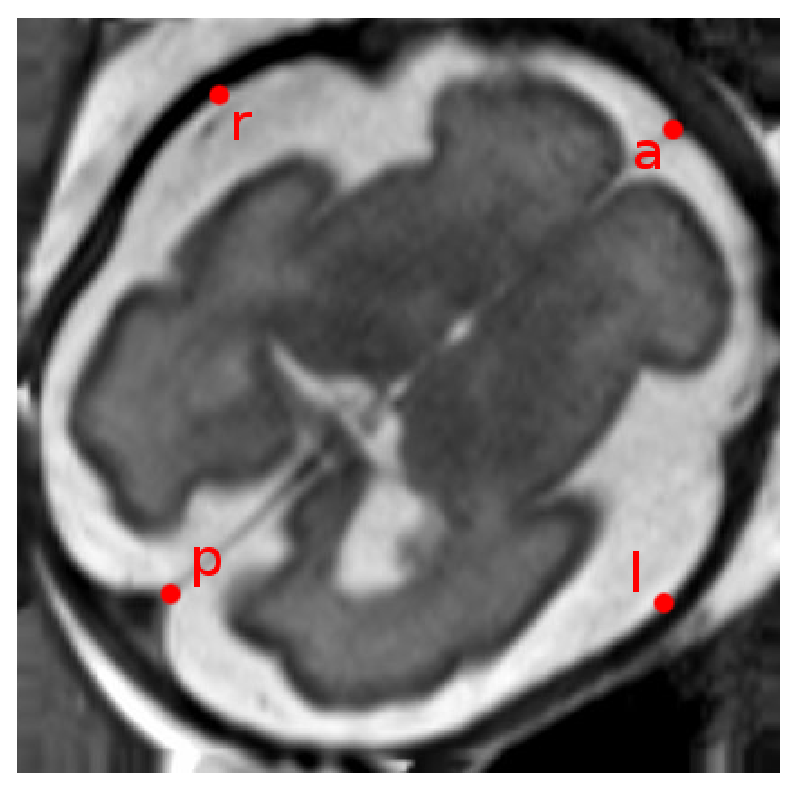
\includegraphics[width=0.35\columnwidth]{lmks_axial.eps}&
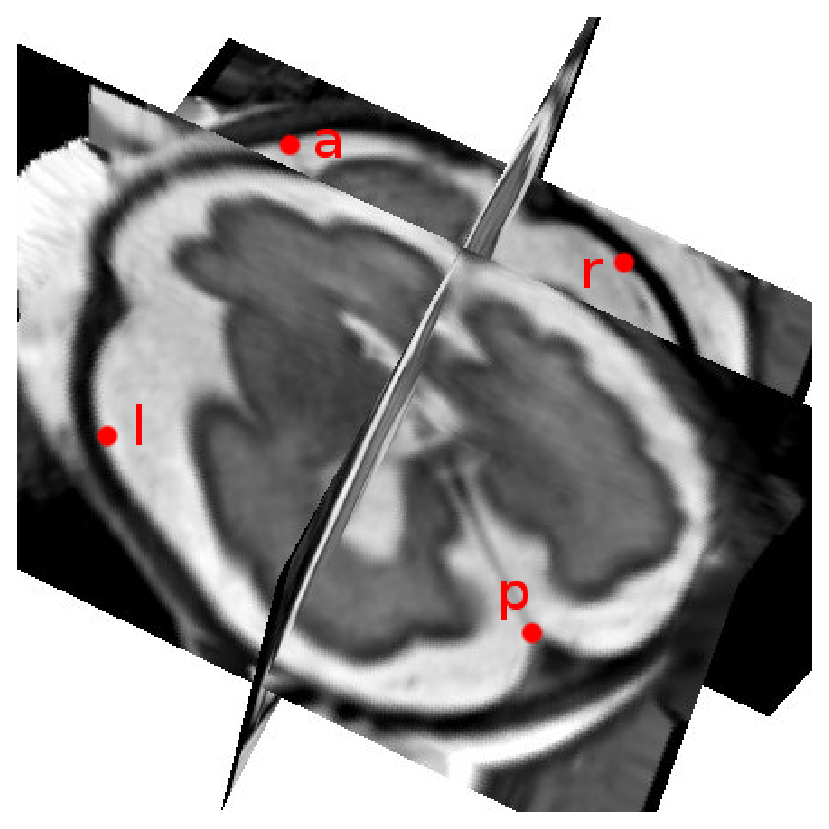
\includegraphics[width=0.35\columnwidth]{lmks_3D.eps}\\
{(a)}&{(b)}\\
\end{tabular}
\caption{Placement of landmarks by using Slicer. (a) axial slice, (b) 3D view.}
\label{fig:landmarks}
\end{figure}

  \item[btkReorientDiffusionSequenceToStandard] Reorients a DW sequence
to the standard orientation. This is necessary with fetal images since the fetus
is in a random orientation with respect to the scanner. This is particularly
important in DWI because colormaps lack of significance, which makes difficult
the identification of specific bundles 

Usage: \texttt{btkReorientDiffusionSequenceToStandard -i image -o output -l
landmarks}.

\texttt{landmarks} is a landmarks file obtained as explained above.

\item[btkCropImageUsingMask] This program crops one (3D or 4D) image using a 3D mask. Usage: \texttt{-i input\_image\_filename -m
input\_mask\_filename -o output\_image\_filename -d 3}, where '-d' is the dimension of the input image (by default 3).

\item[btkRegisterDiffusionToAnatomicalData] This program registers a DW
sequence to an anatomical image. 

Recommended usage: \texttt{btkReorientDiffusionSequenceToStandard -i input
-o output -r reference.nii --mask mask.nii}.
\begin{itemize}
\item[-i] input sequence
\item[-o] resampled sequence (by default, linear interpolation is used)
\item[-r] reference image (anatomical image)
\item[-m] image mask for the B0 image
\end{itemize}

The list of optional parameters can be obtained by \texttt{btkNiftiToNrrd
--help}

\end{description}
